\section{Experiments}
\label{sec:experiments}

We ask three questions.
(Q1)~Does anchoring reduce the bias and MSE of the score target as the theory predicts, including with an imperfect buffer?
(Q2)~Does a less biased target give better samplers in full iDEM-style training?
(Q3)~Where does anchoring fail, and does the failure match \cref{thm:contraction}?
All methods share one codebase, network, noise schedule, test function, proposal count ($K=100$) and training budget (\cref{app:exp}). The only differences are the regression target and, for the explore$\to$anchor variants, the iteration at which the anchor is switched on.

% -------------------------------------------------------------
\subsection{Estimator study (Q1)}
\label{sec:exp-estimator}
For GMM-40 we can sample the posterior $\pi_t(\cdot\mid x_t)$ exactly and evaluate $\nabla\log p_t$ in closed form, so bias and variance can be measured directly.
\Cref{fig:estimator} reports the relative MSE and relative squared bias of each estimator over 12 noise levels, averaged over 256 points and 32 independent repeats. In each repeat the proposals and the anchor are redrawn.
Three findings stand out.
\textbf{(i) With exact anchors, the bias disappears and the MSE drops by orders of magnitude at high noise.}
With TSI at $\sigma_t=70$, the relative MSE falls from $2.4\cdot10^6$ (iDEM, $K=10$) to $5.0\cdot10^3$ (AEM, $K=10$), a $475\times$ reduction. The gain is still $29\times$ at $K=500$.
Even AEM with $K=0$ (pure target score matching on the anchor) beats iDEM with $K=500$ at high noise. Conversely, at low noise ($\sigma_t\le0.25$) the two coincide, as expected: there the proposals already sample the posterior well.
With DSI, iDEM's relative squared bias stays around $7$--$8\cdot10^{-2}$ at $K=10$ for all $\sigma_t\ge2.8$. AEM's is indistinguishable from zero, as \cref{thm:unbiased} predicts.
\textbf{(ii) TSI is the wrong test function at high noise for both methods.} Its relative variance grows like $\sigma_t^2$ because the signal $\nabla\log p_t=O(\sigma_t^{-1})$ shrinks while $\mathrm{Var}[\nabla\mathcal{E}]$ does not. DSI is accurate there but noisy at low noise. This motivates the precision-weighted combination (\cref{sec:method}), which all methods use in \cref{sec:exp-training}. For a unit Gaussian component the combination has zero variance.
\textbf{(iii) Approximate anchors behave as \cref{thm:contraction} predicts.} With tempered anchors (component std $2$ instead of $1$), the bias of AEM at $\sigma_t=2.8$ shrinks geometrically in $K$ ($8.9\cdot10^{-2}$, $2.1\cdot10^{-2}$, $2.5\cdot10^{-3}$, $5\cdot10^{-4}$ for $K=0,10,100,500$). It is already below iDEM's bias at $K\ge10$.
With anchors drawn from a target that lacks half of the modes, the proposals at intermediate noise ($\sigma_t\approx14$) rarely reach the missing modes, so $\epsilon_K$ is small. AEM's bias then \emph{exceeds} iDEM's ($0.16$ vs.\ $0.05$ at $K=10$). This is the buffer-reliance regime we return to in \cref{sec:exp-ablation}.


\begin{figure*}[t]
\centering
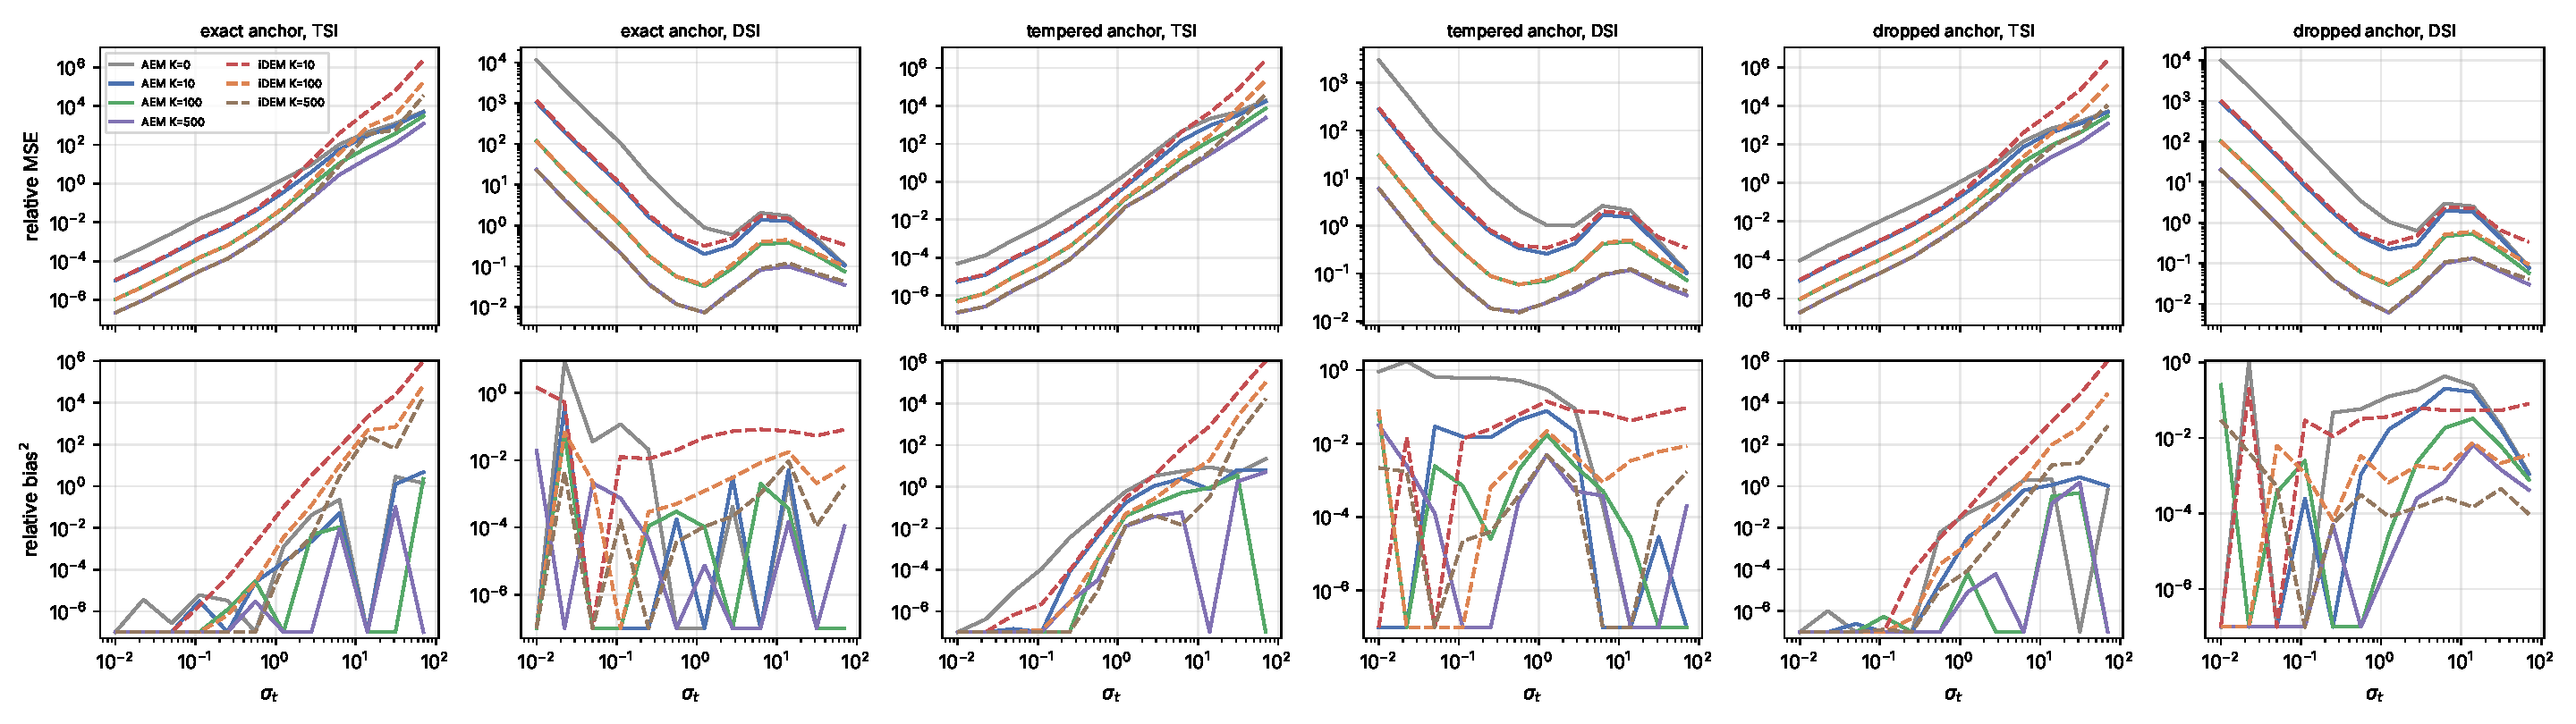
\includegraphics[width=\textwidth]{fig_estimator_gmm40.pdf}
\caption{\textbf{Estimator study on GMM-40.} Relative MSE (top) and debiased relative squared bias (bottom) of the noised-score target against $\sigma_t$, for iDEM (dashed) and AEM (solid) with TSI or DSI test functions. Columns use exact anchors (left), anchors from a tempered target (centre) and anchors from a target missing half of its modes (right). With exact anchors AEM is unbiased for every $K$, including $K=0$. iDEM's bias grows by orders of magnitude with $\sigma_t$.}
\label{fig:estimator}
\end{figure*}

% -------------------------------------------------------------
\subsection{Training samplers (Q2)}
\label{sec:exp-training}
We train on three targets of increasing dimension: GMM-40 ($d=2$), a 10-component Gaussian mixture in $d=16$, and the many-well MW-32 ($d=32$, $2^{16}$ modes).
We compare iDEM, AEM from scratch (\emph{cold}), explore$\to$anchor AEM (iDEM for 20 outer iterations, then anchored targets; the first phase is identical to the iDEM run with the same seed), and explore$\to$anchor AEM with replay proposals (AEM-R).
\Cref{tab:main} reports the final metrics and \cref{fig:curves} the training curves.

\paragraph{iDEM's fixed-point bias is visible, and AEM removes it.}
\Cref{cor:fixed} predicts that iDEM converges to the biased field $b_K$. On MW-32 this bias has a clear signature: the Gaussian coordinates of iDEM samples have variance $4.1\pm0.4$ instead of $1$, and the energy histogram is shifted ($\mathcal{E}$-$\mathcal{W}_1=44.5$). Every AEM variant brings the variance ratio to $1.04$--$1.05$ and lowers $\mathcal{E}$-$\mathcal{W}_1$ by $4$--$29\times$, with a better $\mathcal{W}_2$, at a 1\% higher energy budget.
On GMM-10 ($d=16$) the effect is the same but smaller: the within-mode variance ratio is $1.21$ for iDEM and $1.05$--$1.09$ for AEM, and $\mathcal{E}$-$\mathcal{W}_1$ falls from $1.57$ to $0.29$--$0.62$.
\Cref{fig:marginals} shows the effect directly: iDEM's Gaussian marginals are about twice too wide, its double-well marginals put mass between the wells, and its energy histogram is shifted by about $40$ units. The anchored model matches all three.
These quantities are governed by the within-mode posterior, where the anchor is informative.

\paragraph{In two dimensions there is nothing to fix.}
On GMM-40 all four methods perform similarly ($\mathcal{W}_2$ $4.6$--$5.0$, $\mathcal{E}$-$\mathcal{W}_1$ $0.71$--$0.92$, all 40 modes covered), and most differences are within one standard deviation. This matches the estimator study: in $d=2$, SNIS with $K=100$ is already nearly unbiased at the noise levels that matter. The within-mode variance ratio of $1.7$--$1.9$ is nearly the same for every method, so it reflects the sampler discretization ($\sigma_{\max}/\sigma_{\min}=7000$ with 500 steps) and not the regression target.


\begin{figure*}[t]
\centering
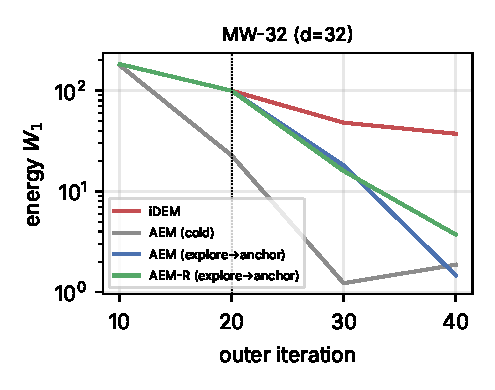
\includegraphics[width=\textwidth]{fig_curves.pdf}
\caption{\textbf{Energy $\mathcal{W}_1$ during training} (mean and min--max over 3 seeds). The dotted line marks the switch from exploration to anchoring in the explore$\to$anchor runs. Before it, those runs coincide with iDEM.}
\label{fig:curves}
\end{figure*}

\begin{figure}[t]
\centering
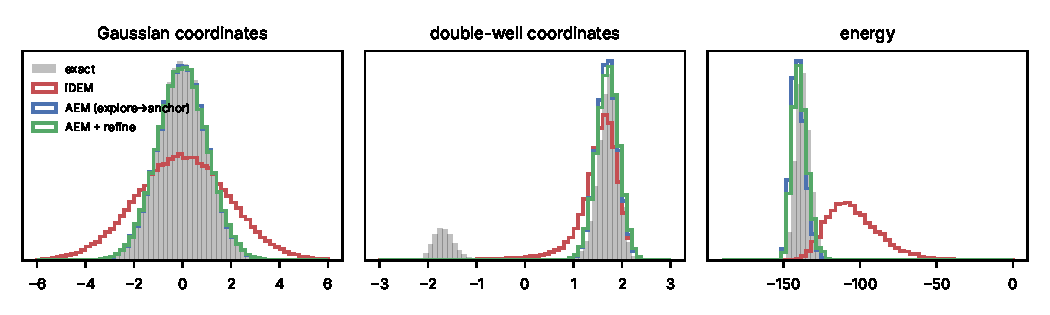
\includegraphics[width=\columnwidth]{fig_mw_marginals.pdf}
\caption{\textbf{MW-32 marginals} (samples pooled over 3 seeds) against exact samples (grey). iDEM's fixed-point bias widens the Gaussian coordinates, smears mass between the wells and shifts the energy distribution. AEM removes these distortions.}
\label{fig:marginals}
\end{figure}

\paragraph{Oracle buffer: testing the fixed point directly.}
To rule out explanations such as short training, the stability caps or the sampler loop, we remove the loop entirely. We train on a \emph{fixed buffer of $10^4$ exact samples} from $\pi$ (\texttt{oracle} mode; rows drawn without replacement), so the buffer law is exactly $\pi$ and \cref{cor:fixed} applies verbatim. We then measure the relative error of the learned score against the exact noised score $\nabla\log p_t$ at $x_t=x_0+\sigma_t\varepsilon$, $x_0\sim\pi$ (\cref{tab:oracle}).
On MW-32 the result is unambiguous. Trained on exact samples, iDEM learns a score whose relative error is $25.0\pm2.6$ at $\sigma_t=1$ and $35.0\pm2.3$ at $\sigma_t=2$ (3 seeds), against $0.140\pm0.003$ and $0.074\pm0.004$ for AEM. Ten times more proposals barely help iDEM: with $K=1000$ (one seed) its error is still $9.8$--$27.6$. This is what one expects from an SNIS bias that decays like $1/K$ with a constant that is exponential in $d$. With a perfect buffer, AEM also gets the mode weights right: in seed 0 the fraction of double-well coordinates in the major well is $0.837$, against a true $0.844$ (iDEM: $0.898$). So the mode-weight deficits of \cref{tab:main} come from the self-generated buffer, as \cref{thm:contraction} predicts, and not from the anchored target.
On GMM-10, where the TSI/DSI combination is exact within each unit-variance component, the two methods learn similar scores at $\sigma_t\ge0.3$ (differences within one standard deviation); AEM is more accurate at $\sigma_t\le0.1$ in the mean.
On the molecular targets we rank the models by held-out denoising loss, which by \cref{prop:diag}(ii) differs between two models by exactly the difference of their score errors (normalized as $\tilde L=\sigma_t^2L/d_{\mathrm{eff}}$; the held-out configurations are disjoint from every seed's buffer). On DW-4 the AEM model has the lower score error at every noise level and in every seed at $\sigma_t\ge0.3$, by a margin that grows from $0.02$ to $10.9$ (\cref{tab:diag}); its samples also have a lower interatomic-distance $\mathcal{W}_1$ in every seed ($0.035$--$0.101$ vs.\ $0.085$--$0.250$). On LJ-13, AEM is better at $\sigma_t\in\{1,2\}$ in all seeds, but slightly worse in the mean at $\sigma_t\le0.3$ (not consistent across seeds), and the gaps are small compared with DW-4. The oracle-trained LJ-13 models of both methods produce some very high-energy samples, so we do not use their sample metrics.



\begin{table*}[t]
\centering
\caption{\textbf{Sampler quality on the synthetic targets} (mean $\pm$ sample std over 3 seeds; $80$ outer iterations; lower is better, except that the variance ratio should be $1$). All methods use the same budget and target function. The variance ratio measures within-mode spread (truth $=1$). Bold marks the best mean in each column (for the variance ratio, the closest to $1$). MMD is the unbiased estimate of MMD$^2$. Mode TV is the total-variation distance between empirical and true mode occupancies (GMM-10: the 10 components; MW-32: the 16 sign patterns of the first four double-well coordinates).}
\label{tab:main}
\small
\begin{tabular}{lccccc}
\toprule
Method & $\mathcal{W}_2$ & $\mathcal{E}$-$\mathcal{W}_1$ & MMD & mode TV & var.\ ratio \\
\midrule
\multicolumn{6}{l}{\textbf{GMM-10 ($d{=}16$)}}\\
iDEM & \textbf{11.6{\scriptsize$\pm$5.6}} & 0.87{\scriptsize$\pm$0.22} & \textbf{0.0138{\scriptsize$\pm$0.018}} & \textbf{0.173{\scriptsize$\pm$0.18}} & 1.12{\scriptsize$\pm$0.027} \\  % n=2
AEM (cold) & 20{\scriptsize$\pm$2} & \textbf{0.125{\scriptsize$\pm$0.079}} & 0.0981{\scriptsize$\pm$0.033} & 0.623{\scriptsize$\pm$0.11} & \textbf{1.02{\scriptsize$\pm$0.013}} \\  % n=2
AEM (explore$\to$anchor) & 14.6{\scriptsize$\pm$3.5} & 0.426{\scriptsize$\pm$0.098} & 0.0309{\scriptsize$\pm$0.021} & 0.286{\scriptsize$\pm$0.18} & 1.06{\scriptsize$\pm$0.013} \\  % n=2
AEM (explore$\to$anchor) + refine & 13.6{\scriptsize$\pm$5} & 0.415{\scriptsize$\pm$0.19} & 0.0258{\scriptsize$\pm$0.027} & 0.275{\scriptsize$\pm$0.2} & 1.06{\scriptsize$\pm$0.026} \\  % n=2
\midrule
\multicolumn{7}{l}{\textbf{MW-32 ($d{=}32$)}}\\
iDEM & 7.74{\scriptsize$\pm$0.17} & 36.4{\scriptsize$\pm$1.5} & \textbf{0.0371{\scriptsize$\pm$0.0048}} & \textbf{0.434{\scriptsize$\pm$0.04}} & 3.67{\scriptsize$\pm$0.22} & 0.974{\scriptsize$\pm$0.0025} \\  % n=2
AEM (cold) & 6.78{\scriptsize$\pm$nan} & \textbf{0.523{\scriptsize$\pm$nan}} & 0.173{\scriptsize$\pm$nan} & 0.481{\scriptsize$\pm$nan} & 1.05{\scriptsize$\pm$nan} & 0.925{\scriptsize$\pm$nan} \\  % n=1
AEM (explore$\to$anchor) & \textbf{6.21{\scriptsize$\pm$0.0051}} & 2.68{\scriptsize$\pm$0.2} & 0.1{\scriptsize$\pm$0.0021} & 0.481{\scriptsize$\pm$0} & \textbf{1.03{\scriptsize$\pm$0.014}} & 1{\scriptsize$\pm$0} \\  % n=2
AEM (explore$\to$anchor) + refine & 6.23{\scriptsize$\pm$0.056} & 1.83{\scriptsize$\pm$0.88} & 0.102{\scriptsize$\pm$0.00041} & 0.481{\scriptsize$\pm$0} & 1.04{\scriptsize$\pm$0.036} & 1{\scriptsize$\pm$0} \\  % n=2
\bottomrule

\end{tabular}
\end{table*}

\begin{table}[t]
\centering
\caption{\textbf{Molecular targets} (mean $\pm$ sample std over 3 seeds; $40$ outer iterations for DW-4, $30$ for LJ-13; EGNN score network). $\mathcal{E}$-$\mathcal{W}_1$: energy-histogram distance; tr: after removing model samples whose energy exceeds the $99.9\%$ quantile of the reference energies (their fraction is in the last column; the reference itself has $0.1\%$); $d$-$\mathcal{W}_1$: $\mathcal{W}_1$ between pooled interatomic distances. Bold marks the best mean per column.}
\label{tab:mol}
\footnotesize
\setlength{\tabcolsep}{3pt}
\begin{tabular}{lcccc}
\toprule
Method & $\mathcal{E}$-$\mathcal{W}_1$ & $\mathcal{E}$-$\mathcal{W}_1^{\mathrm{tr}}$ & $d$-$\mathcal{W}_1$ & frac.\ high-$\mathcal{E}$ \\
\midrule
\multicolumn{5}{l}{\textbf{DW-4 ($d{=}8$)}}\\
iDEM & 1.87{\scriptsize$\pm$0.04} & 0.844{\scriptsize$\pm$0.39} & 0.224{\scriptsize$\pm$0.22} & 0.00224{\scriptsize$\pm$0.0038} \\  % n=3
AEM (explore$\to$anchor) & \textbf{1.85{\scriptsize$\pm$0.008}} & \textbf{0.332{\scriptsize$\pm$0.017}} & \textbf{0.0593{\scriptsize$\pm$0.036}} & \textbf{-5.65e-05{\scriptsize$\pm$0.0001}} \\  % n=2
AEM (explore$\to$anchor) + refine & 1.87{\scriptsize$\pm$0.0013} & 0.635{\scriptsize$\pm$0.16} & 0.142{\scriptsize$\pm$0.13} & 0.000561{\scriptsize$\pm$0.00096} \\  % n=2
\bottomrule

\end{tabular}
\end{table}

% -------------------------------------------------------------
\subsection{Where anchoring fails (Q3)}
\label{sec:exp-ablation}
The same table shows the price of anchoring, and it is the one \cref{thm:contraction} predicts.
When no proposal can reach a mode (high noise, high dimension), $M_t$ is huge and the contraction factor $1-\epsilon_K$ is close to one. The target then follows the buffer: AEM keeps the modes and mode weights the buffer has, and it does not discover new ones.
Started from scratch, AEM inherits whichever modes the first, essentially random, buffers found. On GMM-10 it covers $5$ of $10$ modes (mode TV $0.65$), against $8$ for iDEM (mode TV $0.21$), and its $\mathcal{W}_2$ and MMD are worse accordingly. On MW-32 it occupies the minor wells less evenly than iDEM.
iDEM explores better precisely \emph{because} its target is biased. When SNIS collapses onto the proposal closest to a mode, the resulting field points every noised point towards its nearest low-energy region, which spreads mass across basins whatever the buffer contains.

Exploring first and anchoring afterwards recovers most of iDEM's coverage. On GMM-10 the explore$\to$anchor run keeps all 8 modes iDEM found and still halves $\mathcal{E}$-$\mathcal{W}_1$. It does not recover iDEM's mode-weight accuracy (mode TV $0.35$ vs.\ $0.21$).
Replay proposals were designed to correct mode weights through the energy (\cref{sec:replay}). In our runs they gave the best variance ratio and $\mathcal{W}_2$ on MW-32, but they did not close the mode-weight gap. Used \emph{without} an anchor from the start, they collapse onto the buffer's modes even faster (2 of 10 modes on GMM-10 after 10 iterations; \cref{app:extra}).

The overall picture is consistent. Anchoring makes the target unbiased exactly where the anchor is informative, and it corrects iDEM's systematic within-mode distortion. Mode discovery is a separate problem, and the bias that hurts iDEM's within-mode accuracy is what helps its exploration.
A sampler that wants both needs an exploration mechanism that does not rely on biased targets, such as tempering or annealing across noise levels. Anchoring can be combined with such mechanisms.

